% !TEX program = xelatex

\documentclass[a4paper]{article}
%% Language and font encodings
\usepackage[english]{babel}
\usepackage[utf8x]{inputenc}
\usepackage[T1]{fontenc}
\usepackage{wrapfig}
\usepackage{subcaption}
\usepackage{graphics}
\usepackage{booktabs}
\usepackage{multirow}
\usepackage[table]{xcolor}
\usepackage{amsmath}
\usepackage{amsthm}
\usepackage{amsfonts}
\usepackage{tweaklist}
\usepackage{blindtext}
%% Useful packages
\usepackage{amsmath}
\usepackage{graphicx}
\usepackage[colorinlistoftodos]{todonotes}
\usepackage[colorlinks=true, allcolors=blue]{hyperref}
\usepackage{xeCJK}
\usepackage{url}
%\usepackage{emumerates}
%% Sets page size and margins
\usepackage[a4paper,top=2cm,bottom=2cm,left=1cm,right=3cm,marginparwidth=2cm]{geometry}

\begin{document}
\setlength{\leftskip}{20pt}

\title{2D-Ising模型的临界响应}
\author{仰旗,学号:{\it 201928000807088}}
%%%%% ------------------------ %%%%% 

 \maketitle

% \begin{abstract}
% \end{abstract}
% \tableofcontents
\section{Introduction}
本文简单介绍了Ising模型在临界点处的动力学性质,并结合Metropolis和Heat-Bath更新算法的蒙特卡洛模拟的结果进行了简单的论证。
\newline
2D-Ising模型是统计物理的经典模型,它的定义是:
$$\mathcal{H}=\sum_{\left\langle i,j\right\rangle}-Js_is_j-\sum_ihs_i$$
其中 $s_i$可以取 $+1$ 或 $-1$.
它最核心的性质是,在接近相变点$\beta=\frac{\log(1+\sqrt{2})}{2k_BJ}$的时候,系统的在空间上的关联长度会发散,
其中关联长度的定义是:
$$\xi=\int_{\Omega} |\vec{r}|\left\langle S_i S_{i+\vec{r}} \right\rangle dr$$
而在系统达到平衡时,关联长度发散的形式是:
$$\xi\sim|T-T_c|^{-\nu}$$
关联长度也和支配系统的涨落分布有关系,在平衡态下的临界点,系统中任意尺度的涨落的权重都是一样的,而系统的整体性质完全被临界涨落,也就是系统尺度级别的涨落支配。
越大系统的涨落越难以回归,一般用动力学指数度量$z$度量这种尺度为$L$的涨落回归所需要的时间。
$$\tau\sim L^{z}$$
这里的指数$z$的具体取值,依赖于模拟或模型所使用的动力学的具体形式。不同的更新算法有着不同的$z$值,但是又有相当一部分算法的$z$是相等的。在蒙特卡洛模拟平衡态的情况下,我们总是希望$z$越小越好,
因为小的$z$以为即便系统尺寸很大,物理系统中真实存在的临界慢化也不会很严重,模拟过程中很容易就可以得到统计独立的新构型。
以2D-Ising模型为例,对单个自旋进行更新的算法,例如:Metropolis,Heat-Bath,Glauber 都是$z=2$。而对集团更新算法:Wolff,Swendsen-Wang,$z\approx 0ß$,
对于使用了提升操作,比如Worm等算法,$z$往往各不相同地在$1$左右。
因为在临界点附近关联长度发散的性质,临界点处的弛豫时间:
$$\tau_c\sim \xi^z\sim|T-T_c|^{-z\nu}$$
其中,这个弛豫时间使用的定义是:
$$\tau(\Psi,T)=\int_{0}^{\infty}dt\frac{\Psi(t)}{\Psi(0)}$$
其中$\Psi$是某一个物理量,由于选取的任意性,在这里可以不给出它具体的含义。对系统做小波变换以后对应的分量,就是一个允许的定义。
不同的定义虽然会有不同的系数,但是$\tau$对$T_c$的依赖关系通常是一致的。
在此之前,已经有很多人对2D-Ising模型在临界点上的弛豫进行了研究,其中最为重要的结论是:\textbf{临界系统的弛豫大致分为3个阶段,分别是micro-time regime,short-time regime,long-time regime}。
它们各自所表现出的行为和所受支配的物理规律是有所不同的。形如\textbf{Fig.1}。在刚开始演化的第一个阶段,系统在局部快速地依赖动力学达成平衡,
这个过程出现的临界指数$\theta$和算法密切相关,整个演化被系统局部的动力学性质支配。第二个阶段是发生在系统的关联长度增长的阶段,这时系统正在逐渐地呈现出临界现象。
这个时候的系统出现了局部上的尺度不变性和时间上的自相似性,由重整化群推导出的标度规律已经可以使用:
$$M^{(k)}(t,T-T_c,L,m_0)=b^{-k\beta/\nu}M^{(k)}(b^{-z}t,b^{1/\nu}(T-T_c),b^{-1}L,b^{x_0}m_0)$$
第三个阶段发生在系统的关联长度以及达到了平衡状态下的极限的时候,这个时候由于系统自身尺度的有限,或者温度对有限尺度的偏移,系统的关联长度无法继续增长。
因为临界点附近涨落的发散,系统忘记初始系统的状态,此时系统的演化不再依赖于系统初始的状态,外界系统对系统当前相对于平衡状态的响应等同于对微扰的响应。
这个时候系统物理量服从不依赖初始状态的标度律。
$$O(t,T-T_c,L)=b^{-x}O(b^{-z}t,b^{1/\nu}(T-T_c),b^{-1}L)$$
\section{Method}
本文使用了Python和Julia进行了蒙特卡洛模拟,所有的原始代码和原始数据均发布在GitHub上: 
\url{https://github.com/qiyang-ustc/2d-Ising-Dynamics}
\subsection{Dynamics}
本文模拟的使用的模拟方法是使用了Heat-Bath更新算法,动力学指数$z=2$。
每一步,随机或顺序地选取一个自旋然后利用Heat-Bath方法给出的更新概率进行更新。使用Heat-Bath方法而不是Metropolis的原因是,
Metropolis的更新概率为
$$P_M(s_i\rightarrow -s_i)=min\{1,e^{-2\sum_{j \in \left\langle i,j \right\rangle}\beta Js_js_i}\}$$
而Heat-Bath的更新概率为:
$$P_{HB}(s_i\rightarrow -s_i)=\frac{e^{\sum_{j \in \left\langle i,j \right\rangle}\beta Js_js_i}}{e^{\sum_{j \in \left\langle i,j \right\rangle}\beta Js_js_i}+e^{-\beta J\sum_{j \in \left\langle i,j \right\rangle}s_js_i}}$$
这两种更新概率都满足细致平衡原理,但是相比较于Heat-Bath,Metropolis实际上在更新概率上乘了一个因子。$P_M(s_i\rightarrow -s_i))=P_{HB}(s_i\rightarrow -s_i)/P_{HB}(-s_i\rightarrow s_i)$. 
而这个因子 $P_{HB}(-s_i\rightarrow s_i)$依赖于具体的构型,并加速了更新,这相当于对时间轴进行了重新标度。
考虑到这个因素,Heat-Bath的更新速度更接近真实世界的动力学。
\begin{figure}[h]
    \centering
    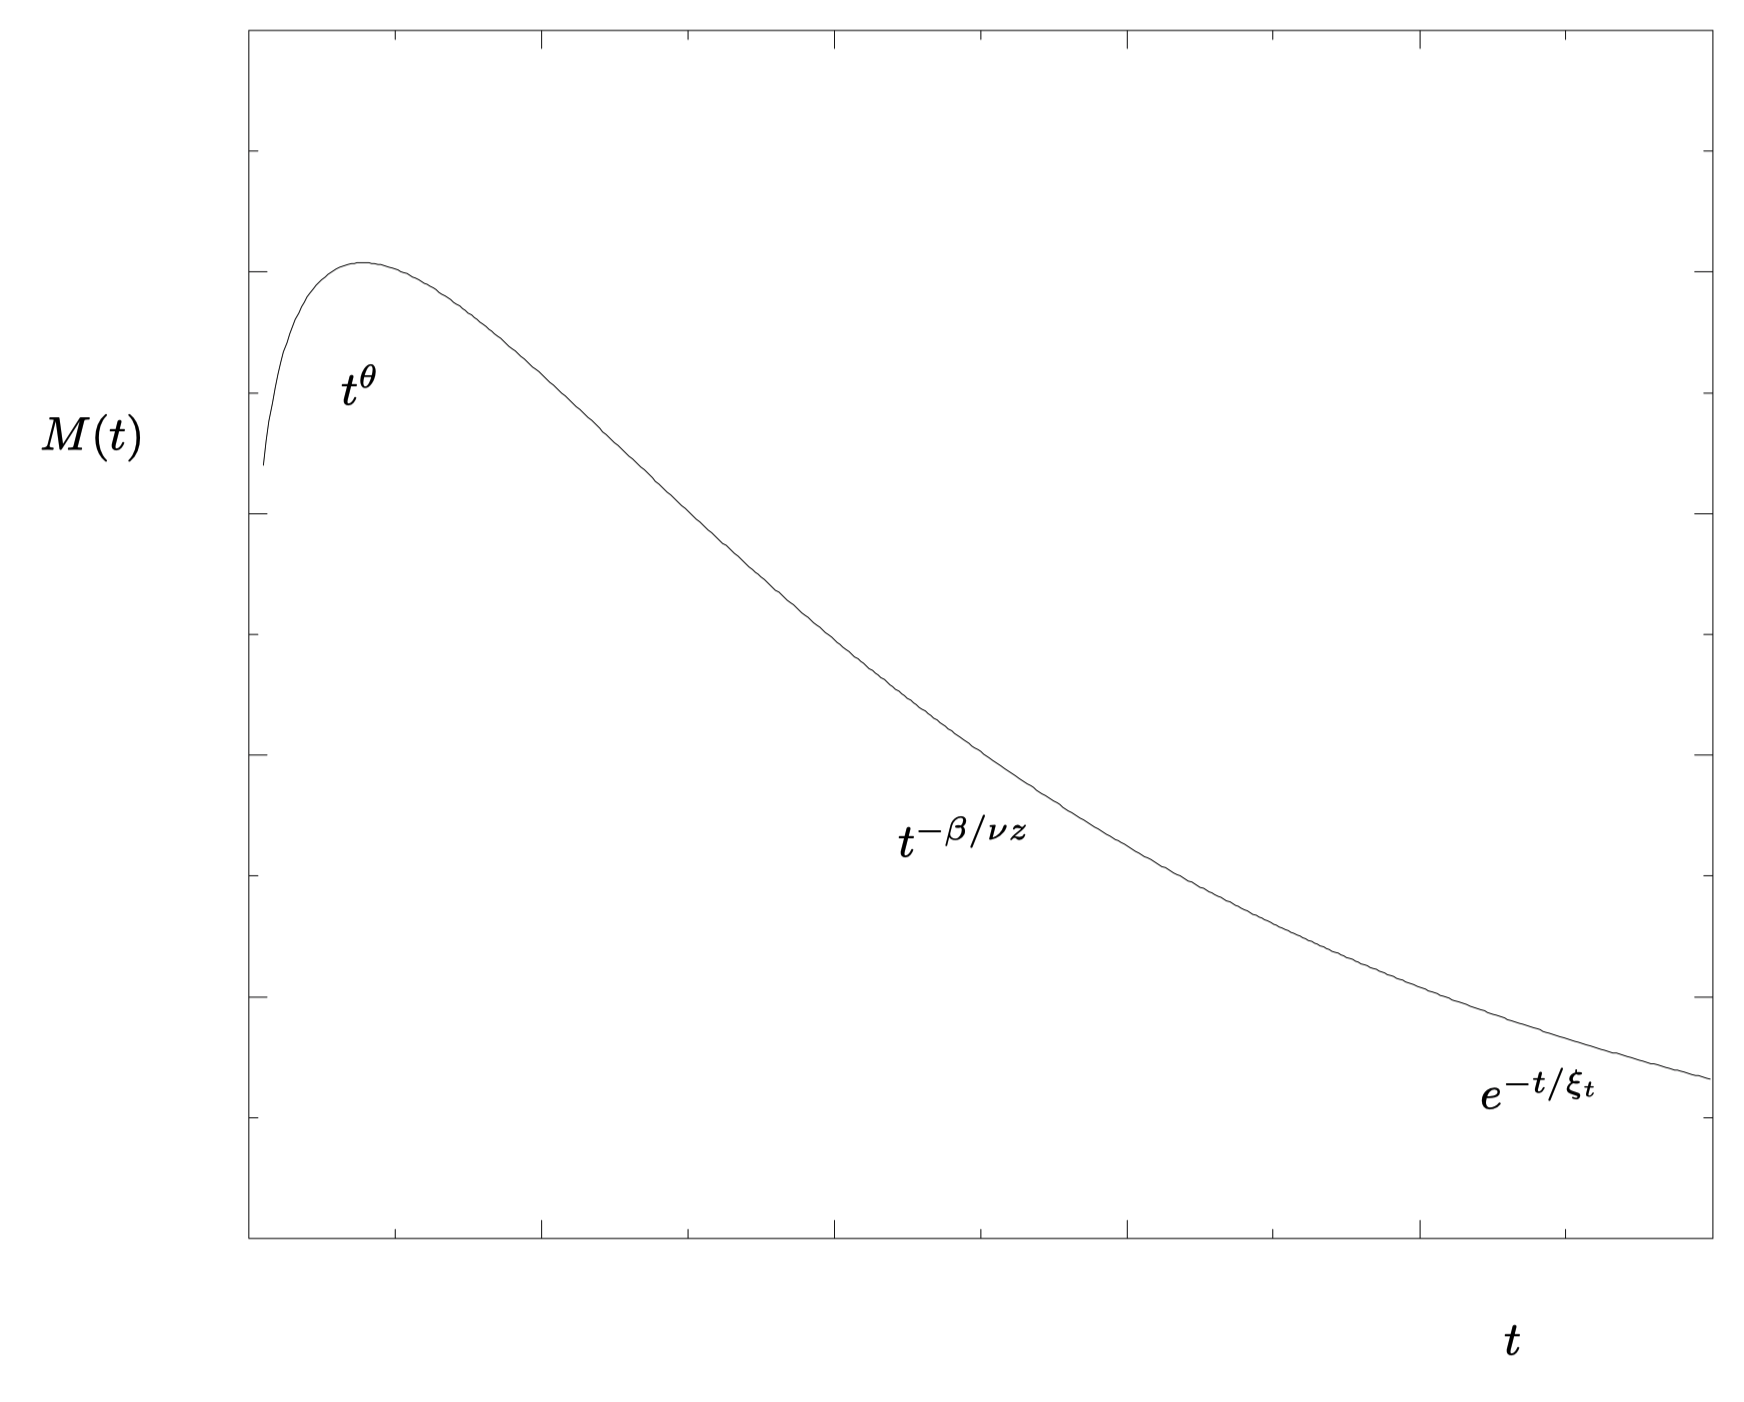
\includegraphics[width=16.0cm]{../figure/sketch.png}
    \caption{高温极限下受磁化系统的弛豫}
\end{figure}


\subsection{System}
我们所模拟的Ising模型的尺寸为$L=8$,$L=16$,$L=32$,$L=64$,先将系统制备在所有自旋向上的状态$\left\langle S_i \right\rangle=1$的状态,
这也恰好对应着$T=0$下系统的一个基态。然后把温度升高到$T_c$附近,这里的$T_c$并未考虑有限尺度修正效应对$T_c$的修正,
所有的$T_c$均选取为$T_c=T_c(L=\infty)$时候的结果,也就是:$\beta=\frac{\log(1+\sqrt{2})}{2k_BJ}\approx 0.4406867935$。
在模拟中,对于每一个$L$,同时作了$log(M(t))\sim log(t)$,$M(t)\sim t$,$log(M(t))\sim t$三幅图,每幅图上有若干条线,每条线标记有相应的$L$
和$dJ$,其中$dJ=\beta J-\beta_c J$,因而也可以看作固定了$J=1$的时候的$\beta-\beta_c$。在模拟过程中,对8192条彼此独立的Markov链进行了1600步的采样。
最终得到的结果如下\textbf{Fig.2}:
\begin{figure}[h]
    \centering
    {
    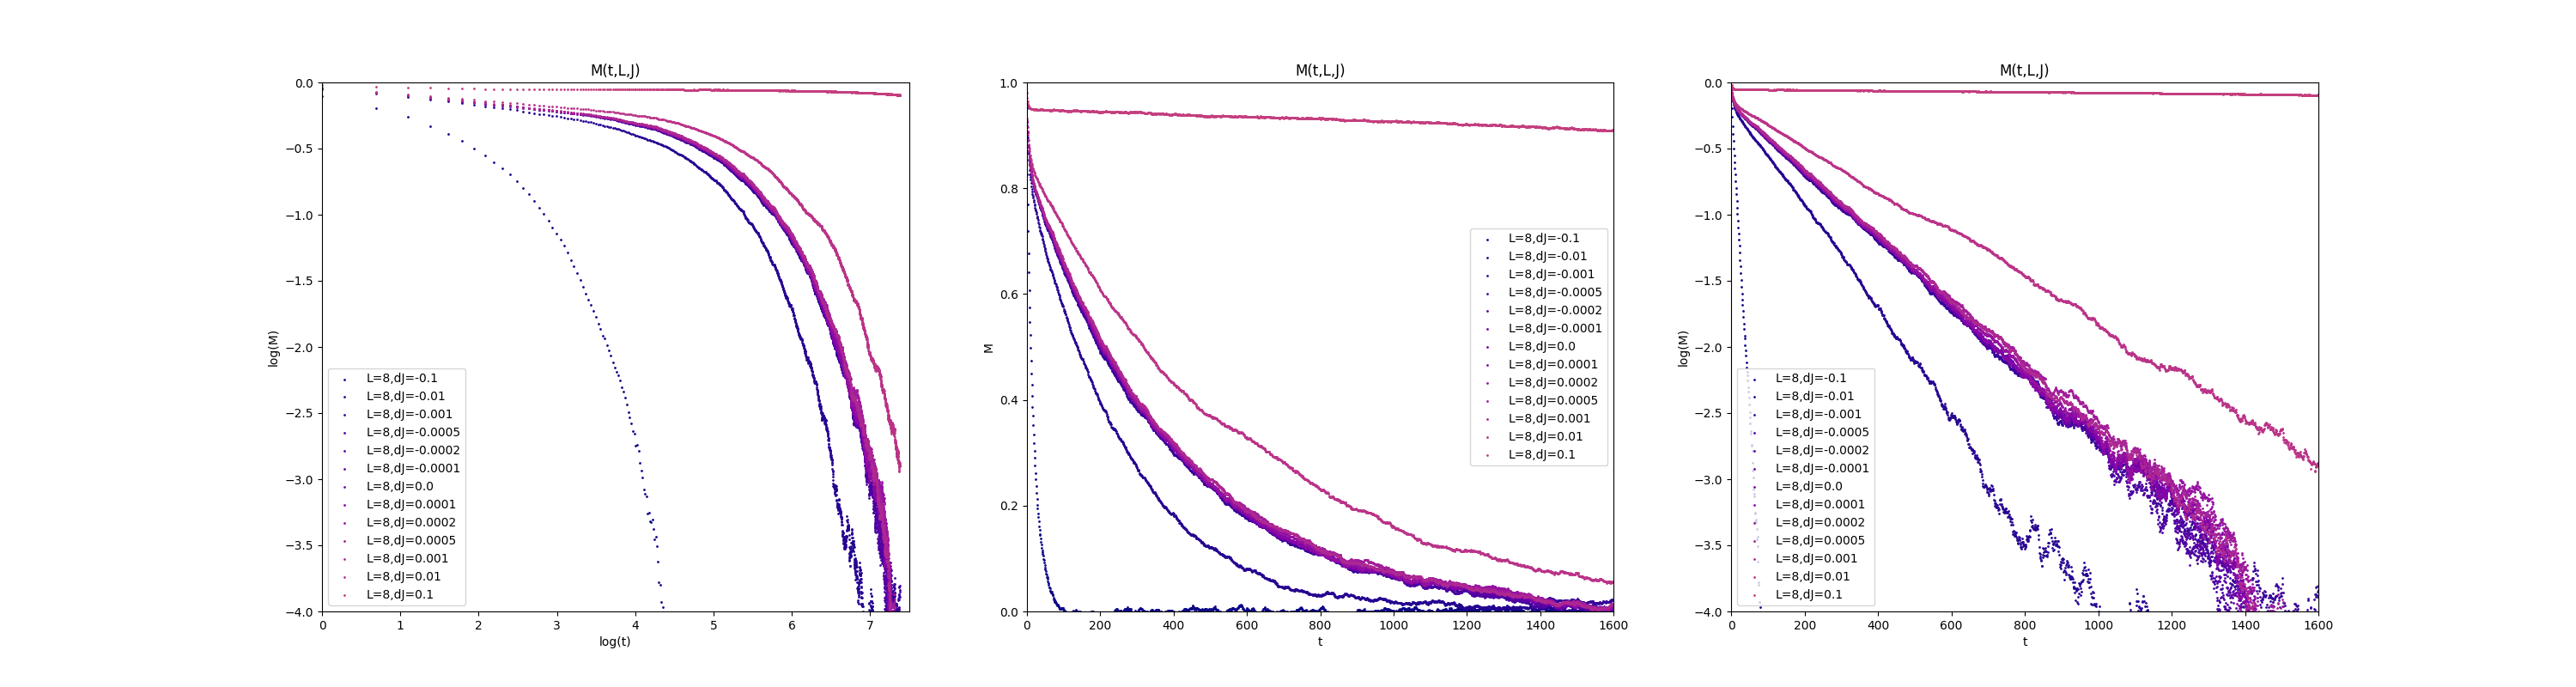
\includegraphics[width=20.0cm]{../figure/fig8.png}}
    \hspace{0in}    %每张图片中间空闲
    {
    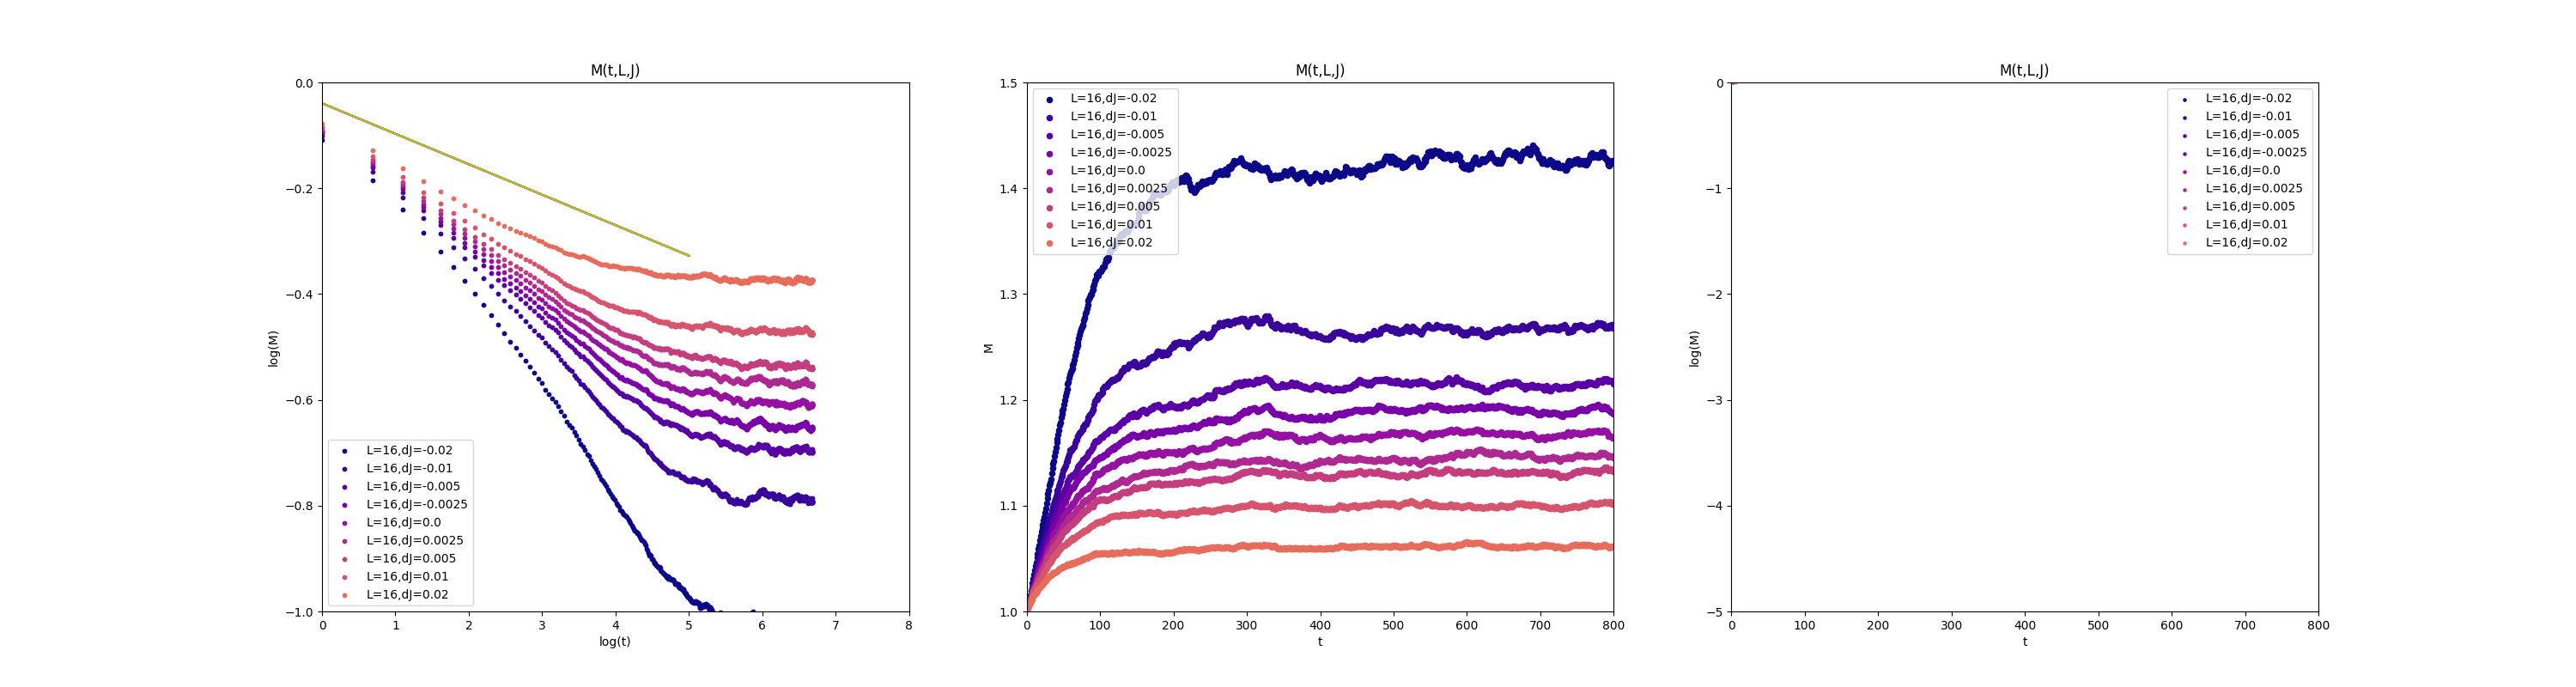
\includegraphics[width=20.0cm]{../figure/fig16.png}}
    \hspace{0in}
    {
    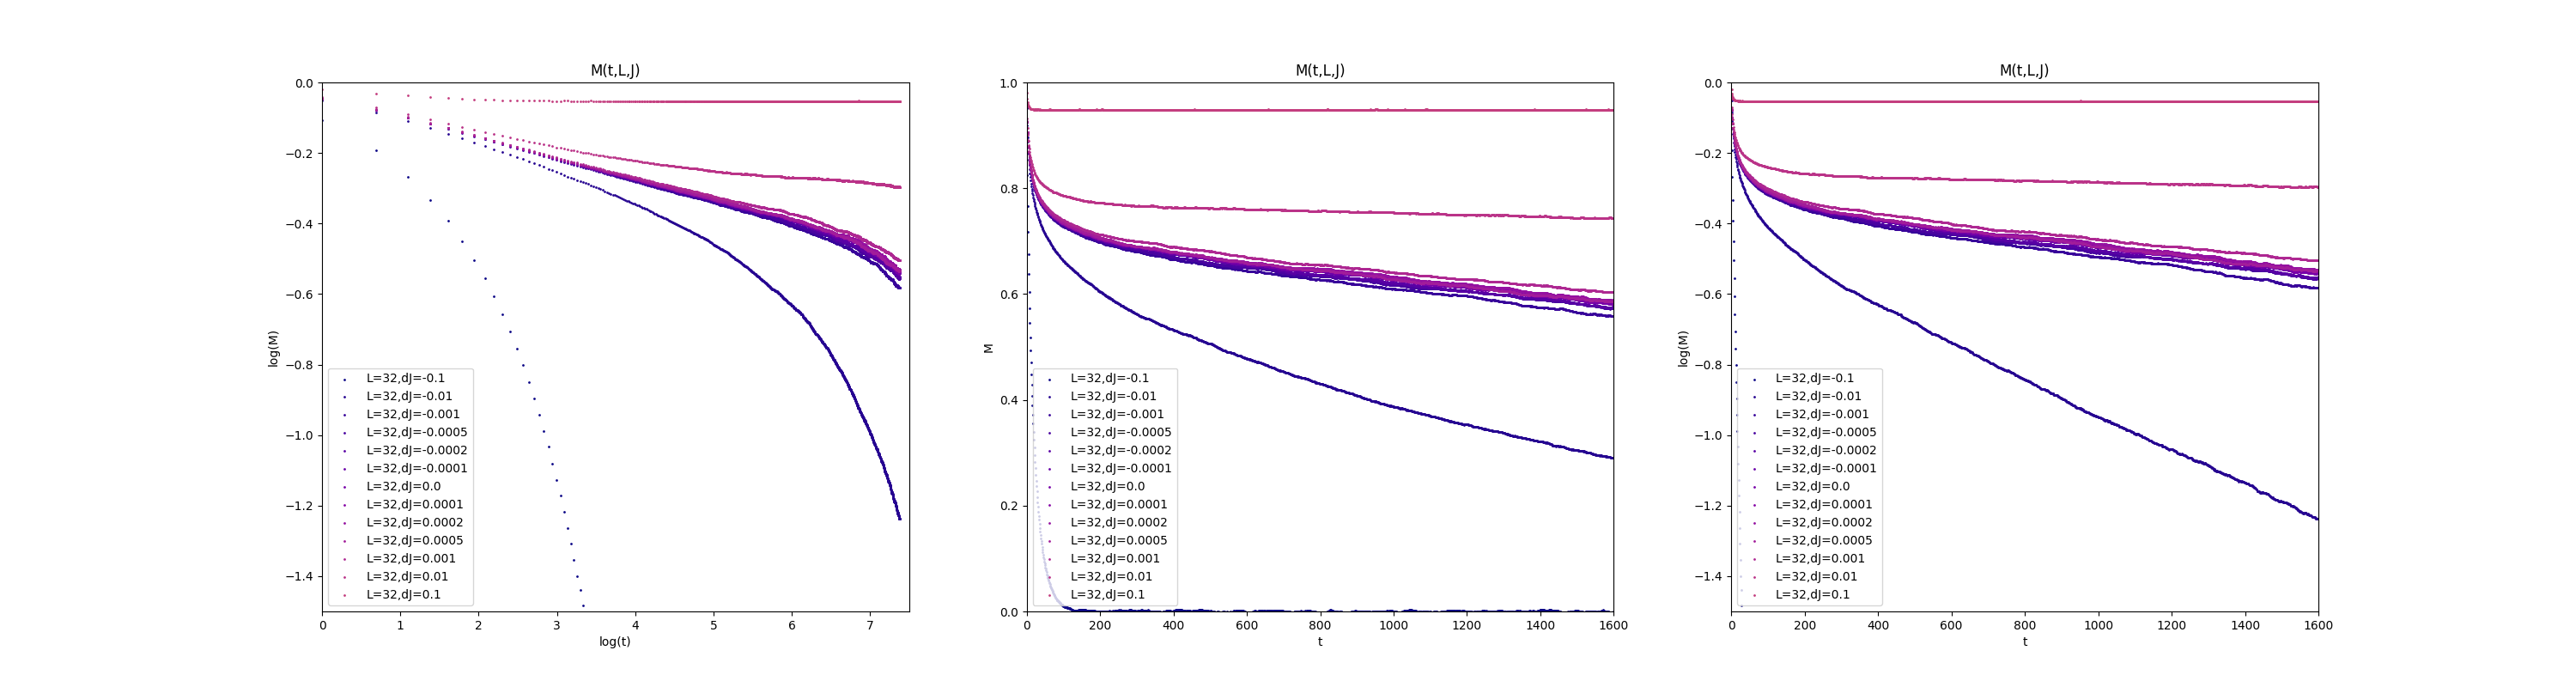
\includegraphics[width=20.0cm]{../figure/fig32.png}}
    \hspace{0in}
    {
    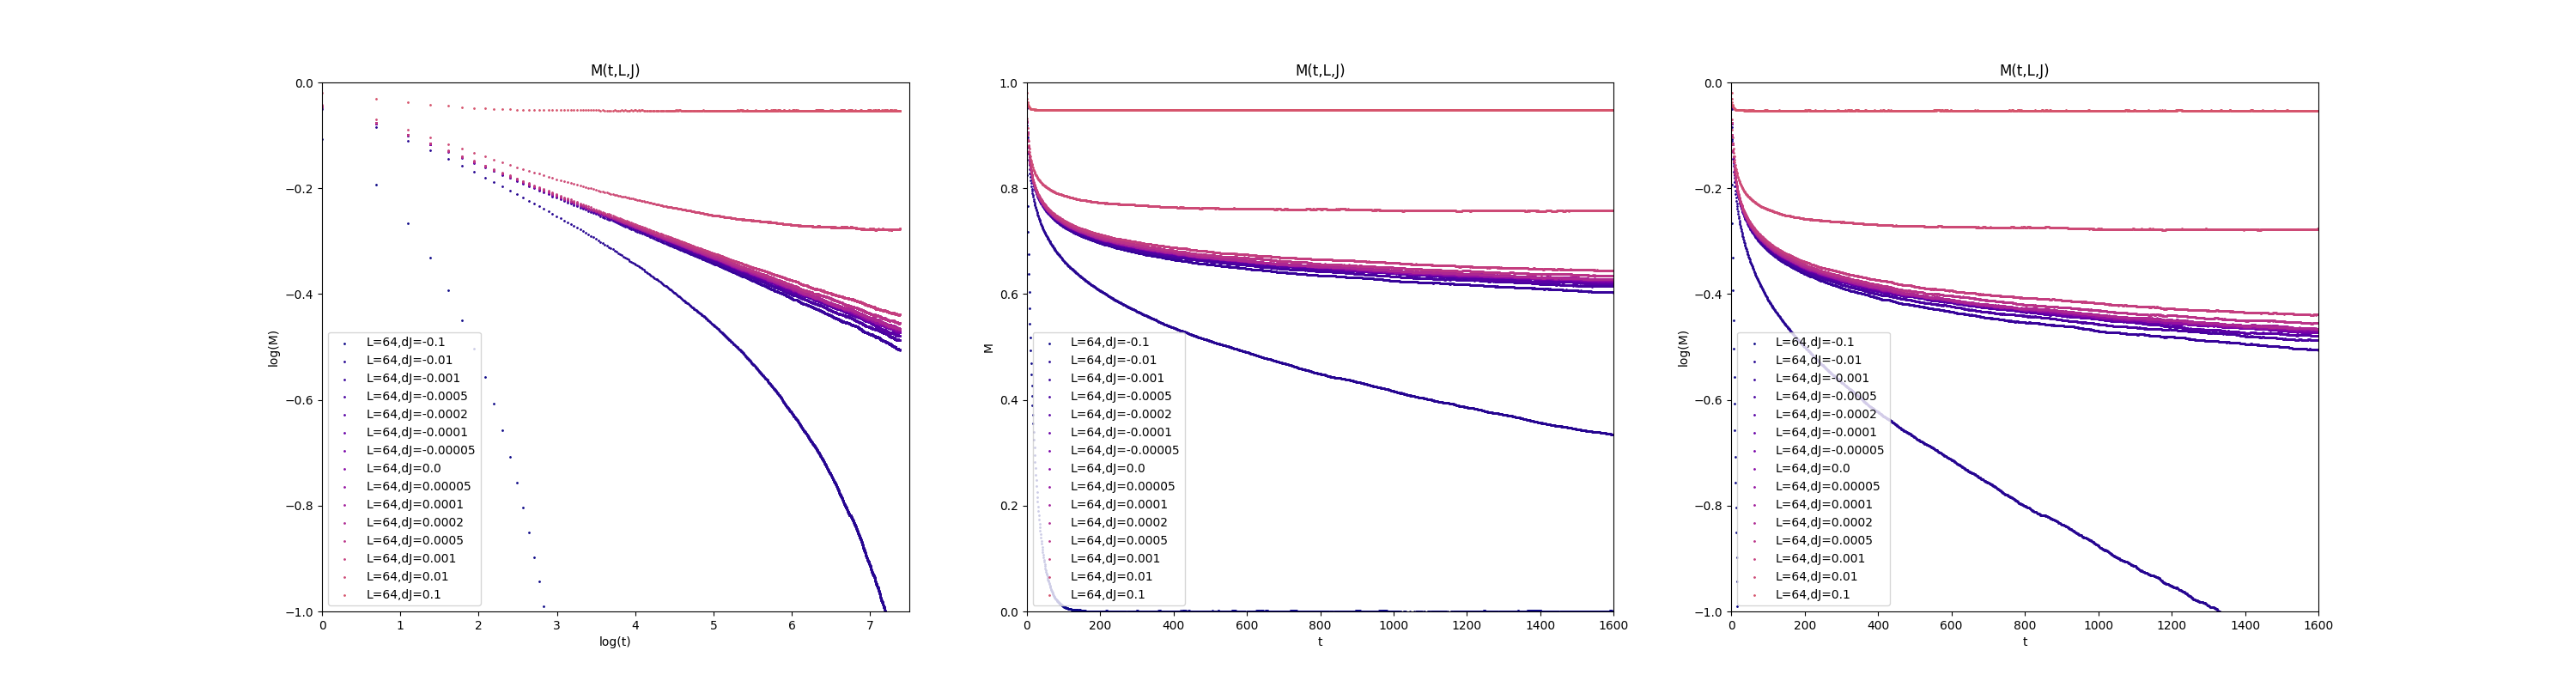
\includegraphics[width=20.0cm]{../figure/fig64.png}}
    \hspace{0in}
    \caption{不同温度,尺寸下,有序态在临界点处演化中:M(t)和t的函数关系}
\end{figure}

\section{Conclusion}
因为我们在所有的模拟中都将系统制备在了有序态,所以无法显著地看到Introduction部分所叙述的系统达到局部平衡的过程,
从结果来看,我们通过改变系统的尺度,成功看到了系统发生的从第二阶段导第三阶段的转变。在$L=8$的系统中我们看到了除了最开始的很小的几步,
系统很快就因为系统的尺寸不够大而进入了由临界涨落所支配的第三阶段,此时,系统的序参量满足的衰减关系已经变成了:$m(t)\sim exp(-t/\tau)$。
因而我们可以在第三列的图中看到直线而无法在第一张图中看到直线。
而对于更大尺寸的系统,我们可以观察到,这个转变发生的时间在不断地推迟,在$L=64$的情况下,1600步的演化已经无法让系统走出short-time regime。
此时,系统的序参量的弛豫所满足的规律是$m(t)\sim t^{-\beta/\nu z}$,所以我们可以清楚地看到系统在第一列的图中呈直线而在第三张图中呈现曲线。
在转变发生的过程中,我们大致可以看到系统在第一列的图中渐渐偏离过原点的直线,而第三列的图中渐渐呈现了直线。
这样的结果符合我们在Introduction的结论。\newline
总的来说,本文写作相对仓促,尤其是受制于个人课程论文不应使用组内计算机集群,在个人Laptop上运行蒙特卡罗计算程序比较吃力。
鉴于程序的基本框架已经搭好,很多后续工作可以低成本地小改程序进行尝试。比如将系统改为自旋玻璃系统,使用其他更新算法等等。
本文最开始的选题动机是,意识到临界点附近因为临界涨落的存在,就算已经被完全磁化,系统回归平衡态的速度应该是比较平凡的,因为系统在平衡态下就已经是无限磁化态。
所以这个弛豫只相当于撤去了一个无限小的磁场,撤去这样的一个微扰的系统理应可以被线性响应理论很好地描述。在仔细思考和模拟确认之后发现,
因为临界涨落的存在,系统的弛豫恰恰非常复杂,线性响应理论一样会失效,尤其是short-time regime的弛豫并不服从通常意义下的线性响应理论。
因为这里的对涨落的响应,并不是只研究对序参量涨落的响应就能很好地刻画的。系统对涨落的响应,是和涨落的动量谱有深刻的依赖的。
本文所进行的研究,实际上只是研究了有限尺度系统对长波极限涨落的响应,而出现在本文中最主要的参考文献:\url{http://arxiv.org/abs/cond-mat/9910504},
在Ising模型上也只研究了长波极限和短波极限,后续的很多工作如果基于的系统对不同动量涨落的响应进行分析,
如果可以把这个弛豫囊括进线性响应理论的框架下,应该是非常有意思的。
% The dynamics in this project is given by Heat Bath Method. Each steps, we pick up a spin sequentially or randomly.
% The reason of using Heat Bath updating instead of Metropolis is a little subtle:
% The differece between Heat Bath and Metropolis is, in Metropolis, the probability of updating is:
% $$P_M(s_i\rightarrow -s_i)=min\{1,e^{-2\sum_{j \in \left\langle i,j \right\rangle}\beta Js_js_i}\}$$
% While the probability of updating in Heat Bath is:
% $$P_{HB}(s_i\rightarrow -s_i)=\frac{e^{\sum_{j \in \left\langle i,j \right\rangle}\beta Js_js_i}}{e^{\sum_{j \in \left\langle i,j \right\rangle}\beta Js_js_i}+e^{-\beta J\sum_{j \in \left\langle i,j \right\rangle}s_js_i}}$$
% Though these two methods both satisfy Detailed Balance, comparing to Heat Bath, Metropolis expand the probability of 
% updating by a const: $P_M(s_i\rightarrow -s_i))=P_{HB}(s_i\rightarrow -s_i)/P_{HB}(-s_i\rightarrow s_i)$. 
% And $P_{HB}(-s_i\rightarrow s_i)$ is configuration depended. Metropolis actually accelerate the updating, what it does 
% is equivalent to rescale time-axis.



% \section{Theoretical analysis}
% The Hamiltonian of oußr system is: $s_i$ could be $+1$ or $-1$.
% $$\mathcal{H}=\sum_{\left\langle i,j\right\rangle}-Js_is_j-\sum_ihs_i$$
% We first prepare our system at $h\rightarrow\infty$, which is equivalent to say:
% $$\mathcal{H} = \mathcal{H}_0-Nhm\theta(-t)$$
% where N is the number of total spins and m is order parameter $m=\sum s_i/N$. T is time. $\theta(t)=1$ if $t>0$ else $theta(t)=0$
% It is obvious that the expectation for order parameter is zero for non-disturbed state.
% And the system is prepare at $m(0)=1$.\newline
% Now, we use linear response theory to analyze this system: when $t=0$, The wight is 
% $$W(x,t=0) = \frac{e^{-\beta H}}{Z}=\frac{e^{-\beta H_0}\times e^{\beta Nmh}}{\sum_{s}e^{-\beta H_0+\beta Nmh}}$$
% So,
% $$=\frac{e^{-\beta H_0}(1+\beta Nhm)}{Z}-\frac{e^{-\beta H_0}}{Z^2}e^{-\beta H_0}Nhm=W_0(x,0)\times(1+\beta Nh(m-\left\langle m\right\rangle))$$
% We can conclude that:
% $$\rho(t=0)+\Delta\rho(t=0)=W(x,0)=W_0(x,0)(1+\beta Nh\delta m) $$
% $$\Delta\rho(t) = \beta NH\delta mW_0(t)$$
% If we donated the time-correlation of order parameter by $A(t)$ which means:
% $$A(t)=\left\langle\delta m(t)\delta m(0)\right\rangle$$
% Generalized susceptibility $\chi$ in linear response theory:
% $$\left\langle \delta m(t)\right\rangle=\int_{\infty}^{t}\chi(t-t')\theta(-t')Nhdt'$$
% Besides, by definition
% $$\left\langle \delta m(t)\right\rangle=Tr(\Delta\rho(t)\hat{m})=Tr(\Delta\rho(0)\hat{m}(t))=\beta Nh \left\langle m(t)m(0)\right\rangle=\beta NhA(t)$$
% Take derivatives of the equation:
% $$\beta NhA(t)=\left\langle m(t)\right\rangle=\int_{-\infty}^{t}\chi(t-t')Nh\theta(-t')dt'$$
% We can get:
% $$\chi(t)= -\beta\dot{A}(t)\quad if\quad t>0$$



% -----------------------------------Appendix----------------------------------------
%\newpage
% -----------------------------------REFERENCE----------------------------------------
\bibliographystyle{alpha}
% \bibliography{sample}
\end{document}